
\section{Vorwort}
\label{vorwort}
	\begin{multicols}{2}
	\subsection*{Willkommen in der Informatik!}	

	Ein neues Semester hat begonnen und wieder strömen unzählige neue Gesichter auf den Campus um das Abenteuer Studium zu beginnen oder fortzusetzen. Da das nicht immer ganz einfach ist haben wir, die Fachgruppe Informatik für die Erstsemester unserer Fachrichtung einen kleinen Leitfaden zusammengestellt - die 1-te.

	Auf den folgenden Seiten werden wir hoffentlich einige der typischen Fragen beantworten, die einen am Anfang des Studiums quälen. Außerdem möchten wir natürlich uns, die Fachgruppe vorstellen (s. Seite \pageref{fachgruppe}) und eventuell noch die ein oder andere hilfreiche Information mitgeben. 

	\subsubsection*{Aufbau dieses Heftes}
		In der ersten Hälfte dieses Heftes sind wichtige
		Erklärungen zum Studienbeginn, dem Studiengang und der
		universitären Infrastruktur. Weitere Informationen zu
		uns und unserer Gremienarbeit, sowie weitere
		Informationen sind in der zweiten Hälfte.
\columnbreak
	\subsubsection*{Die Fachgruppe Online}
		Natürlich gibt es uns auch online - auf der Seite \url{http://fginfo.cs.tu-bs.de}. Beispielsweise stehen dort aktuelle Termine wie Spiele- oder Grillabende. Auch gibt es dort noch einmal die Inhalte dieses Heftes, samt den Aktualisierungen die erst nach dem Druck bekannt wurden. 

	\vspace*{0.5cm}

	Viel Spaß und Erfolg im  Studium wünscht  die\\
	\hspace*{2cm}Fachgruppe Informatik
	\end{multicols}
	\vspace{0.5cm}
	\begin{center} 
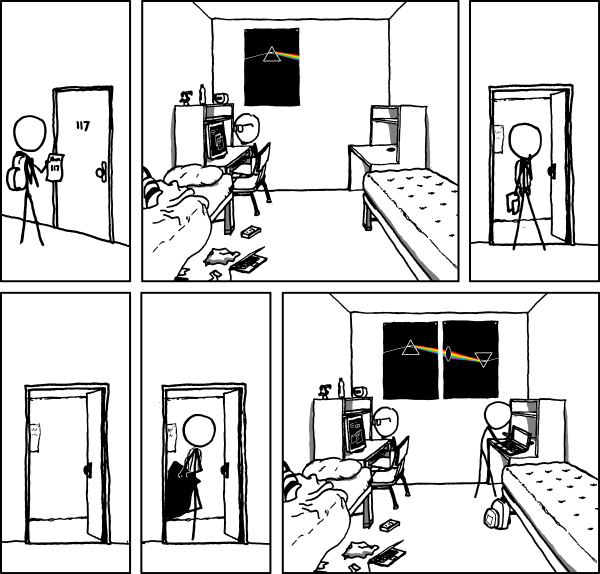
\includegraphics[totalheight=12cm]{bilder/XKCD/dorm_poster}
\end{center}
